%http://www.tablesgenerator.com/latex_tables

%Para el análisis de las rutas nos centraremos principalmente en el RTT y ZRTT de cada Gateway atravesado. Es importante mencionar que no todos los Gateways emiten una respuesta a los paquetes ICMP emitidos ya que algunos podrían no tener implementada esa funcionalidad. Por esta razón se verá más adelante que los TTL presentados en las tablas no crecen de a uno.

%Para calcular el RTT de cada Gateway envíamos numerosos paquetes al mismo para obtener un promedio. Determinamos que envíar 20 paquetes por cada salto era suficiente. También se calculó el desvío estandar:
%\newline
%\newline
%$RTT=\frac{\sum_{i=1}^{20}{RTT_i}}{20}$
%\newline
%$\sigma = \frac{\sum_{i=1}^{20}{(RTT_i-RTT)^2}}{20}$
%\newline

%Además del RTT se obtuvo el ZRTT para cada Gateway. Este valor nos permite analizar si un determinado Gateway tiene un RTT mayor o menor a la media con respecto a la ruta global, dependiendo de si el ZRTT es positivo o negativo. Por lo tanto es una muy buena herramienta para analizar si se trata de un enlace submarino. Fue calculado de la siguiente manera:
%\newline
%\newline
%$ZRTT_i = \frac{RTT_i-\overline{RTT}}{SRTT}$
%en donde $RTT_i$ es el $RTT$ promedio calculado para cada salto, $\overline{RTT}$ es el $RTT$ promedio de la ruta global y $SRTT$ es el desvío estándar de la ruta global.
%\newline

%Para verificar si los valores de RTT y ZRTT se corresponden con la realidad decidimos utilizar una herramienta de geolocalización de modo que podamos determinar la ubicación aproximada de un Gateway. De esta forma nos era posible verificar, por ejemplo, si a valores grandes de ZRTT para determinado Gateway le correspondia una ubicación alejada de nuestro origen. También incluimos, para cada ruta analizada, un mapa en donde pueden verse los lugares por donde van pasando los paquetes.

%A continuación, los resultados obtenidos:

Para cada una de las universidades mencionadas en la sección anterior recopilamos muestras en dos rangos horarios distintos para lograr un análisis más preciso. Haciendo uso de esta información encontraremos un umbral que permita caracterizar lo mejor posible los enlaces submarinos. A continuación, los resultados obtenidos:

\subsection{Universidad de Australia}

% Please add the following required packages to your document preamble:
% \usepackage{graphicx}
\begin{table}[H]
\resizebox{\textwidth}{!}{%
\begin{tabular}{lllllll}
TTL & IP              & RTT(prom)        & RTT Relativo      & ZRTT                  & Fecha            & Lugar                   \\
1   & 192.168.1.1     & 4.50524161844 ms & 4.50524161844 ms  & -0.2816859003457402   & 2014-07-14 22:17 & *                       \\
2   & 190.245.25.1    & 111.661064625 ms & 107.155823006 ms  & 1.4383568281840526    & 2014-07-14 22:17 & Argentina               \\
6   & 200.89.165.49   & 46.1213350296 ms & -65.5397295952 ms & -1.4553796269426058   & 2014-07-14 22:17 & Argentina               \\
7   & 200.89.165.250  & 70.5515384674 ms & 24.4302034378 ms  & 0.05218250283679886   & 2014-07-14 22:17 & Argentina               \\
8   & 64.209.94.97    & 106.063258648 ms & 35.5117201805 ms  & 0.23786759138391753   & 2014-07-14 22:17 & United States           \\
9   & 67.17.106.162   & 233.08006525 ms  & 127.016806602 ms  & 1.7711531938156388    & 2014-07-14 22:17 & United States           \\
10  & 64.208.27.102   & 239.12910223 ms  & 6.04903697968 ms  & -0.25581762030733124  & 2014-07-14 22:17 & United States           \\
11  & 129.250.3.172   & 241.938555241 ms & 2.80945301056 ms  & -0.3101010230336      & 2014-07-14 22:17 & United States:Englewood \\
13  & 129.250.2.168   & 293.335330486 ms & 51.3967752457 ms  & 0.5040421525784031    & 2014-07-14 22:17 & United States:Englewood \\
14  & 129.250.2.230   & 294.001984596 ms & 0.666654109955 ms & -0.3460063790273647   & 2014-07-14 22:17 & United States:Englewood \\
15  & 204.1.253.166   & 273.278772831 ms & -20.7232117653 ms & -0.7044211367972472   & 2014-07-14 22:17 & United States:Englewood \\
16  & 202.158.194.172 & 408.931684494 ms & 135.652911663 ms  & 1.9158622593874055    & 2014-07-14 22:17 & Australia               \\
17  & 113.197.15.68   & 350.345873833 ms & -58.5858106613 ms & -1.3388577569701294   & 2014-07-14 22:17 & Australia               \\
18  & 113.197.15.66   & 457.67967701 ms  & 107.333803177 ms  & 1.441339115228246     & 2014-07-14 22:17 & Australia               \\
19  & 113.197.15.65   & 477.138209343 ms & 19.4585323334 ms  & -0.031124251164705886 & 2014-07-14 22:17 & Australia               \\
20  & 202.158.193.146 & 467.447268963 ms & -9.6909403801 ms  & -0.5195612176543029   & 2014-07-14 22:17 & Australia               \\
21  & 202.158.193.186 & 453.81141901 ms  & -13.6358499527 ms & -0.5856632594872633   & 2014-07-14 22:17 & Australia               \\
22  & 137.111.189.4   & 379.369139671 ms & -74.4422793388 ms & -1.6045533164129089   & 2014-07-14 22:17 & Australia               \\
23  & 137.111.13.200  & 440.604770184 ms & 61.2356305122 ms  & 0.6689048472601429    & 2014-07-14 22:17 & Australia:Ryde          \\
24  & 137.111.223.12  & 489.401388168 ms & 48.7966179848 ms  & 0.46047316807592487   & 2014-07-14 22:17 & Australia               \\
25  & 137.111.223.158 & 447.635984421 ms & -41.7654037476 ms & -1.0570101706073296   & 2014-07-14 22:17 & Australia              
\end{tabular}
}
\caption{Ruta hacia la universidad de Australia. Fecha: 2014-07-14 22:17}
\label{my-label}
\end{table}

% Please add the following required packages to your document preamble:
% \usepackage{graphicx}
\begin{table}[h]
\resizebox{\textwidth}{!}{%
\begin{tabular}{lllllll}
TTL & IP              & RTT(prom)        & RTT Relativo       & ZRTT             & Fecha            & Lugar                   \\
1   & 192.168.1.1     & 3.92243266106 ms & 3.92243266106 ms   & -0.156988637511  & 2014-07-15 11:29 & *                       \\
2   & 190.245.25.1    & 14.4544005394 ms & 10.5319678783 ms   & -0.0683795333018 & 2014-07-15 11:29 & Argentina               \\
6   & 200.89.165.49   & 17.3185110092 ms & 2.86411046982 ms   & -0.171176773023  & 2014-07-15 11:29 & Argentina               \\
7   & 200.89.165.250  & 17.6531434059 ms & 0.334632396698 ms  & -0.205087597129  & 2014-07-15 11:29 & Argentina               \\
8   & 64.209.94.97    & 18.6506390572 ms & 0.997495651245 ms  & -0.196201084346  & 2014-07-15 11:29 & United States           \\
9   & 67.17.106.162   & 303.711605072 ms & 285.060966015 ms   & 3.61202579094    & 2014-07-15 11:29 & United States           \\
10  & 64.208.27.102   & 138.994526863 ms & -164.717078209 ms  & -2.41781265937   & 2014-07-15 11:29 & United States           \\
11  & 129.250.3.172   & 144.09160614 ms  & 5.09707927704 ms   & -0.141241027281  & 2014-07-15 11:29 & United States:Englewood \\
12  & 129.250.3.174   & 174.553048611 ms & 30.4614424706 ms   & 0.198800053905   & 2014-07-15 11:29 & United States:Englewood \\
13  & 129.250.2.168   & 182.045078278 ms & 7.4920296669 ms    & -0.109133715391  & 2014-07-15 11:29 & United States:Englewood \\
14  & 129.250.2.230   & 185.058188438 ms & 3.01311016083 ms   & -0.169179245404  & 2014-07-15 11:29 & United States:Englewood \\
15  & 204.1.253.166   & 184.148418903 ms & -0.909769535065 ms & -0.221770364801  & 2014-07-15 11:29 & United States:Englewood \\
16  & 202.158.194.172 & 304.84919548 ms  & 120.700776577 ms   & 1.40857143673    & 2014-07-15 11:29 & Australia               \\
17  & 113.197.15.68   & 305.96446991 ms  & 1.11527442932 ms   & -0.194622112198  & 2014-07-15 11:29 & Australia               \\
18  & 113.197.15.66   & 327.852737904 ms & 21.8882679939 ms   & 0.0838659041302  & 2014-07-15 11:29 & Australia               \\
19  & 113.197.15.65   & 339.838087559 ms & 11.9853496552 ms   & -0.0488951288643 & 2014-07-15 11:29 & Australia               \\
20  & 202.158.193.146 & 339.18466568 ms  & -0.653421878815 ms & -0.218333703154  & 2014-07-15 11:29 & Australia               \\
21  & 202.158.193.186 & 339.751029015 ms & 0.566363334656 ms  & -0.201980953446  & 2014-07-15 11:29 & Australia               \\
22  & 137.111.189.4   & 342.869663239 ms & 3.11863422394 ms   & -0.16776456307   & 2014-07-15 11:29 & Australia               \\
23  & 137.111.13.200  & 341.519153118 ms & -1.35051012039 ms  & -0.227679044787  & 2014-07-15 11:29 & Australia:Ryde          \\
24  & 137.111.223.12  & 381.63330555 ms  & 40.1141524315 ms   & 0.328206729975   & 2014-07-15 11:29 & Australia               \\
25  & 137.111.223.158 & 343.915832043 ms & -37.7174735069 ms  & -0.715223772604  & 2014-07-15 11:29 & Australia              
\end{tabular}
}
\caption{Ruta hacia la universidad de Australia. Fecha: 2014-07-15 11:29}
\label{my-label}
\end{table}

%Notar que a medida que los TTL's se van incrementando también lo hacen el RTT y ZRTT. Esto era esperado que sucediera ya que los Gateways se encuentran cada vez más lejos del origen. Este comportamiento podrá verse mejor en los siguientes gráficos.

\begin{figure}[H]
	\begin{center}
		  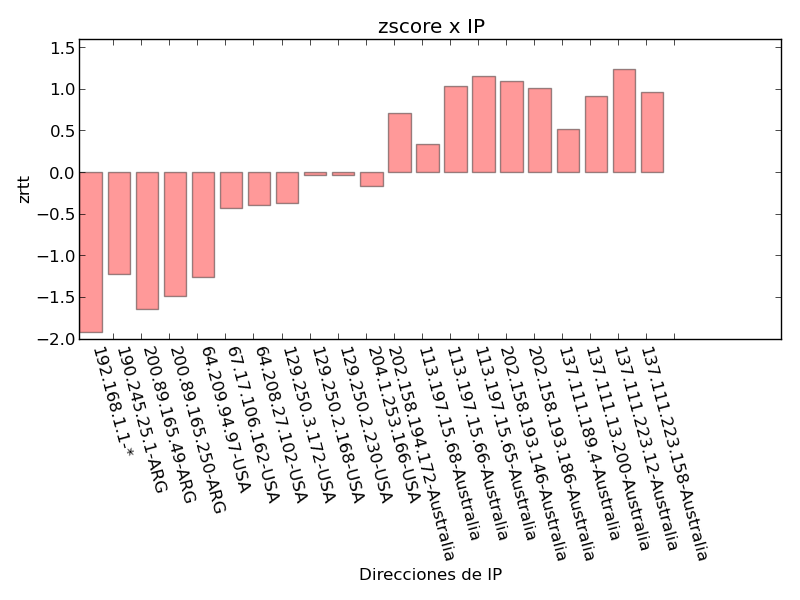
\includegraphics[scale=0.5]{../graficos_informe/mq_zscore.png}
		  \caption{ZRTT para cada Gateway. Fecha: 2014-07-14 22:17}
		  \label{fig:contra1}
	\end{center}
\end{figure}

\begin{figure}[H]
	\begin{center}
		  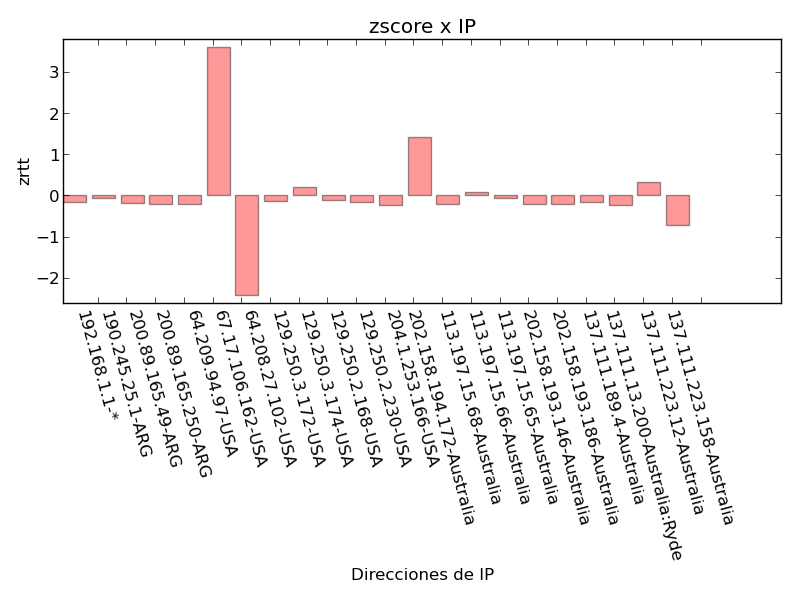
\includegraphics[scale=0.5]{../graficos_informe/mq_zscore_segunda_medicion.png}
		  \caption{ZRTT para cada Gateway. Fecha: 2014-07-15 11:29}
		  \label{fig:contra1}
	\end{center}
\end{figure}

%Aquí puede observarse claramente que a partir del Gateway que se encuentra localizado en Australia, el ZRTT se torna positivo. Esto indica, como mencionamos anteriormente, que el RTT para estos Gateways es mayor a la media de la ruta global lo cual tiene sentido ya que atraviesan un enlace submarino.

%\begin{figure}[H]
%	\begin{center}
%		  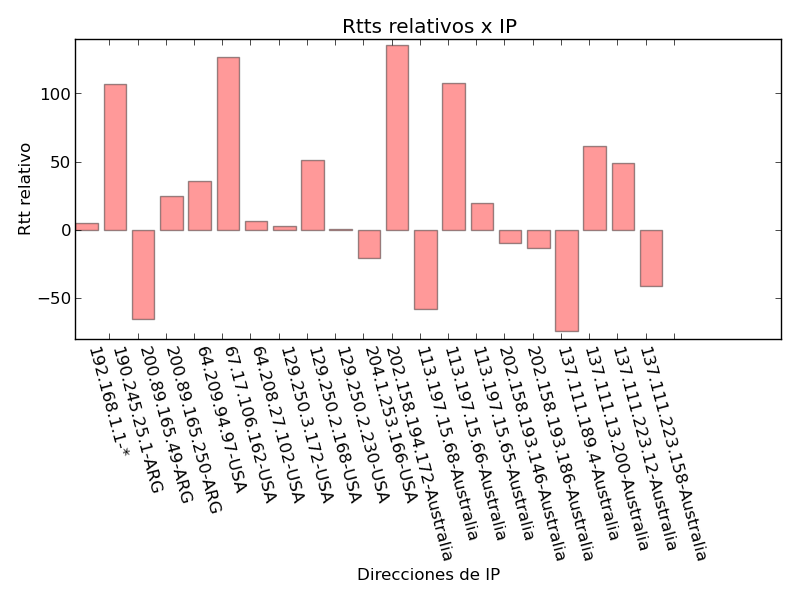
\includegraphics[scale=0.5]{../graficos_informe/mq_rtt.png}
%		  \caption{RTT relativo para cada Gateway}
%		  \label{fig:contra1}
%	\end{center}
%\end{figure}

%Podemos ver en este gráfico que los RTT's van creciendo a medida que vamos hacia la derecha del gráfico.

\begin{figure}[H]
	\begin{center}
		  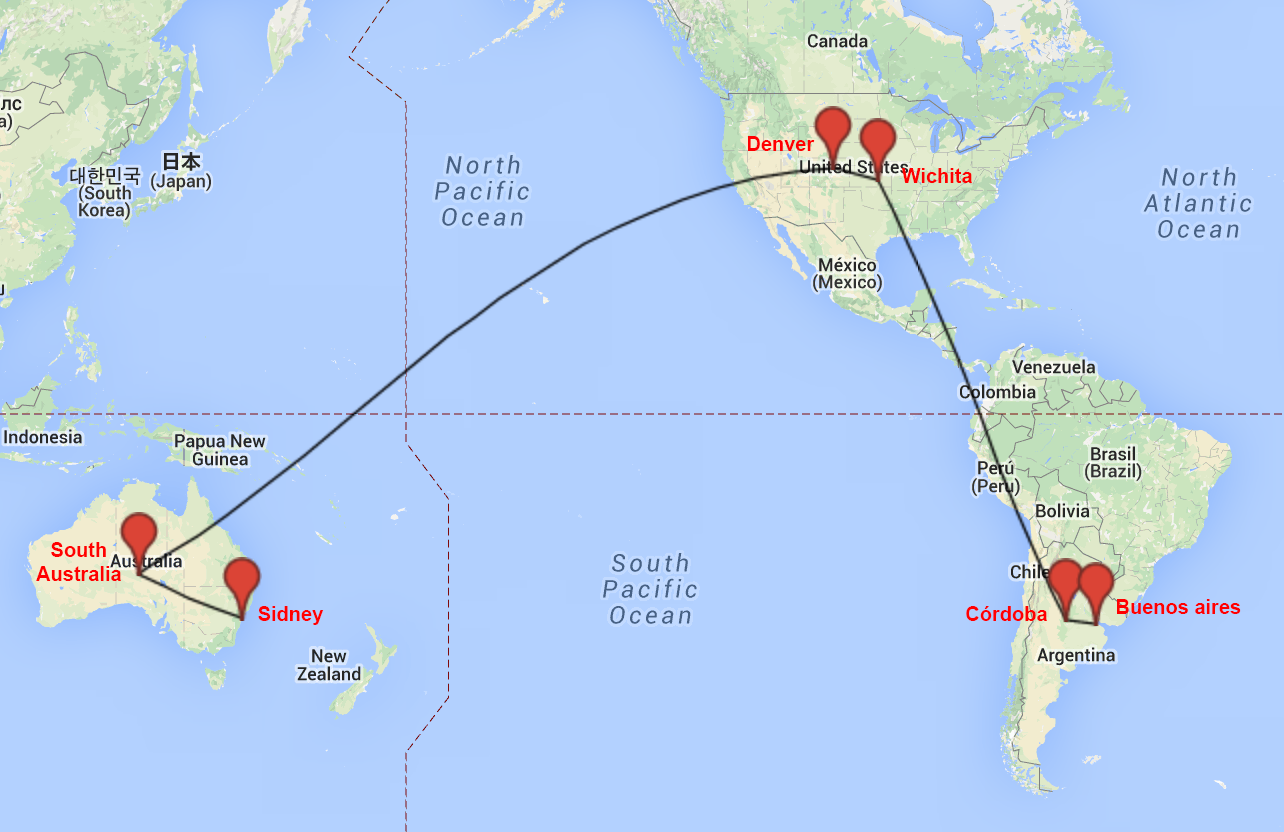
\includegraphics[scale=0.4]{../mapas/mapa_md.png}
		  \caption{Mapa de la ruta atravesada para llegar a la universidad de Australia}
		  \label{fig:contra1}
	\end{center}
\end{figure}

\subsection{Universidad de Kamchatka}

% Please add the following required packages to your document preamble:
% \usepackage{graphicx}
\begin{table}[H]
\resizebox{\textwidth}{!}{%
\begin{tabular}{lllllll}
TTL & IP             & RTT(prom)        & RTT Relativo      & ZRTT                 & Fecha            & Lugar                        \\
1   & 192.168.1.1    & 4.09276783466 ms & 4.09276783466 ms  & -0.40164567614243346 & 2014-07-14 22:26 & *                            \\
2   & 190.245.25.1   & 40.4574036598 ms & 36.3646358252 ms  & -0.16957636692760783 & 2014-07-14 22:26 & Argentina                    \\
6   & 200.89.165.13  & 34.34227705 ms   & -6.1151266098 ms  & -0.4750513746584941  & 2014-07-14 22:26 & Argentina                    \\
7   & 200.89.165.2   & 65.1411771774 ms & 30.7989001274 ms  & -0.2095999701178342  & 2014-07-14 22:26 & Argentina                    \\
8   & 200.89.165.86  & 109.000182152 ms & 43.8590049744 ms  & -0.11568382274747024 & 2014-07-14 22:26 & Argentina                    \\
9   & 195.22.220.174 & 82.8942418098 ms & -26.1059403419 ms & -0.6188067449646265  & 2014-07-14 22:26 & Italy                        \\
10  & 89.221.34.255  & 300.520706177 ms & 217.626464367 ms  & 1.133890397036675    & 2014-07-14 22:26 & Italy                        \\
11  & 195.22.214.27  & 292.13514328 ms  & -8.38556289673 ms & -0.4913782442676092  & 2014-07-14 22:26 & Italy                        \\
12  & 95.167.93.6    & 449.580430984 ms & 157.445287704 ms  & 0.7011232544587561   & 2014-07-14 22:26 & Russian Federation           \\
13  & 213.59.5.6     & 413.960599899 ms & -35.6198310852 ms & -0.6872218132646754  & 2014-07-14 22:26 & Russian Federation           \\
14  & 213.59.5.17    & 950.969684124 ms & 537.009084225 ms  & 3.4305936429533395   & 2014-07-14 22:26 & Russian Federation           \\
15  & 213.59.5.18    & 956.076347828 ms & 5.10666370392 ms  & -0.39435467848267897 & 2014-07-14 22:26 & Russian Federation           \\
16  & 85.28.192.173  & 954.074466228 ms & -2.00188159943 ms & -0.44547273581218666 & 2014-07-14 22:26 & Russian Federation           \\
17  & 85.28.192.90   & 949.170184135 ms & -4.90428209305 ms & -0.46634410519857006 & 2014-07-14 22:26 & Russian Federation           \\
18  & 77.82.16.83    & 955.445873737 ms & 6.2756896019 ms   & -0.3859481296991383  & 2014-07-14 22:26 & Russian Federation:Kamchatka \\
19  & 85.28.217.202  & 959.138429165 ms & 3.69255542755 ms  & -0.4045236321654454  & 2014-07-14 22:26 & Russian Federation          
\end{tabular}
}
\caption{Ruta hacia la universidad de Kamchatka. Fecha: 2014-07-14 22:26}
\label{my-label}
\end{table}

% Please add the following required packages to your document preamble:
% \usepackage{graphicx}
\begin{table}[h]
\resizebox{\textwidth}{!}{%
\begin{tabular}{lllllll}
TTL & IP             & RTT(prom)        & RTT Relativo       & ZRTT            & Fecha            & Lugar                        \\
1   & 192.168.1.1    & 3.89574468136 ms & 3.89574468136 ms   & -0.397745899903 & 2014-07-15 11:35 & *                            \\
2   & 190.245.25.1   & 15.3007745743 ms & 11.4050298929 ms   & -0.343778553071 & 2014-07-15 11:35 & Argentina                    \\
6   & 200.89.165.13  & 16.6796326637 ms & 1.37885808945 ms   & -0.415834131714 & 2014-07-15 11:35 & Argentina                    \\
7   & 200.89.165.2   & 16.1038756371 ms & -0.575757026672 ms & -0.429881459645 & 2014-07-15 11:35 & Argentina                    \\
8   & 200.89.165.86  & 19.2112088203 ms & 3.10733318329 ms   & -0.403412015327 & 2014-07-15 11:35 & Argentina                    \\
9   & 195.22.220.174 & 21.3767766953 ms & 2.16556787491 ms   & -0.410180246071 & 2014-07-15 11:35 & Italy                        \\
10  & 89.221.34.255  & 270.991384983 ms & 249.614608288 ms   & 1.36817385969   & 2014-07-15 11:35 & Italy                        \\
11  & 195.22.214.27  & 263.068211079 ms & -7.92317390442 ms  & -0.482685499416 & 2014-07-15 11:35 & Italy                        \\
12  & 95.167.93.6    & 401.302981377 ms & 138.234770298 ms   & 0.567714937488  & 2014-07-15 11:35 & Russian Federation           \\
13  & 213.59.5.6     & 404.476010799 ms & 3.17302942276 ms   & -0.402939872954 & 2014-07-15 11:35 & Russian Federation           \\
14  & 213.59.5.17    & 937.531983852 ms & 533.055973053 ms   & 3.40519576096   & 2014-07-15 11:35 & Russian Federation           \\
15  & 213.59.5.18    & 936.572170258 ms & -0.959813594818 ms & -0.432641577744 & 2014-07-15 11:35 & Russian Federation           \\
16  & 85.28.192.173  & 932.444596291 ms & -4.12757396698 ms  & -0.455407475944 & 2014-07-15 11:35 & Russian Federation           \\
17  & 85.28.192.90   & 938.281881809 ms & 5.83728551865 ms   & -0.38379253353  & 2014-07-15 11:35 & Russian Federation           \\
18  & 77.82.16.83    & 938.936829567 ms & 0.654947757721 ms  & -0.421036693456 & 2014-07-15 11:35 & Russian Federation:Kamchatka \\
19  & 85.28.217.202  & 947.841417789 ms & 8.9045882225 ms    & -0.361748599361 & 2014-07-15 11:35 & Russian Federation          
\end{tabular}
}
\caption{Ruta hacia la universidad de Kamchatka. Fecha: 2014-07-15 11:35}
\label{my-label}
\end{table}

\begin{figure}[H]
	\begin{center}
		  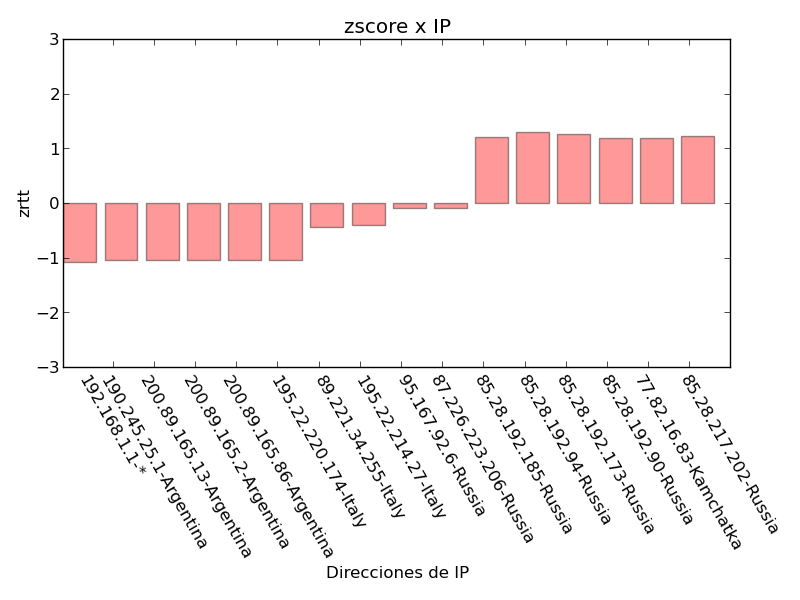
\includegraphics[scale=0.5]{../graficos_informe/kamgu_zscore.png}
		  \caption{ZRTT para cada Gateway. Fecha: 2014-07-14 22:26}
		  \label{fig:contra1}
	\end{center}
\end{figure}

\begin{figure}[H]
	\begin{center}
		  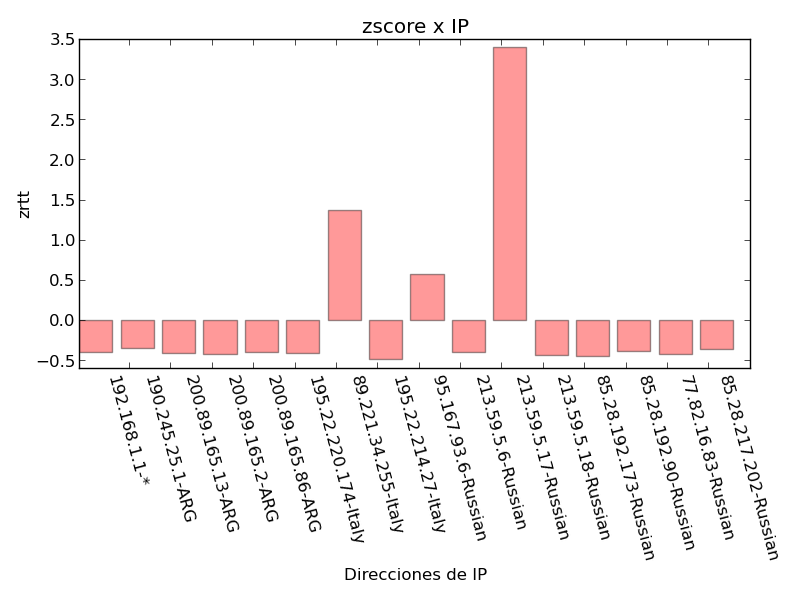
\includegraphics[scale=0.5]{../graficos_informe/kamgu_zscore_segunda_medicion.png}
		  \caption{ZRTT para cada Gateway. Fecha: 2014-07-15 11:35}
		  \label{fig:contra1}
	\end{center}
\end{figure}

%En este caso notamos que el ZRTT se torna positivo recién cuando el paquete atraviesa Rusia y no Italia. Sin embargo, notamos un aumento progresivo del ZScore.

%\begin{figure}[H]
%	\begin{center}
%		  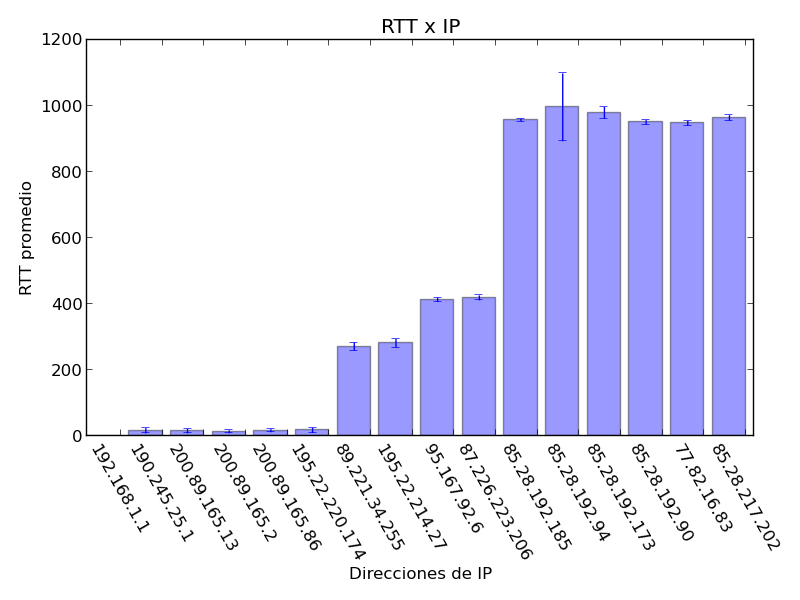
\includegraphics[scale=0.5]{../graficos_informe/kamgu_rtt.png}
%		  \caption{RTT relativo para cada Gateway}
%		  \label{fig:contra1}
%	\end{center}
%\end{figure}

%Al igual que antes, puede observarse un crecimiento hacia la derecha. Notar la gran diferencia que hay entre los RTT's de un Gateway argentino y uno ruso.

\begin{figure}[H]
	\begin{center}
		  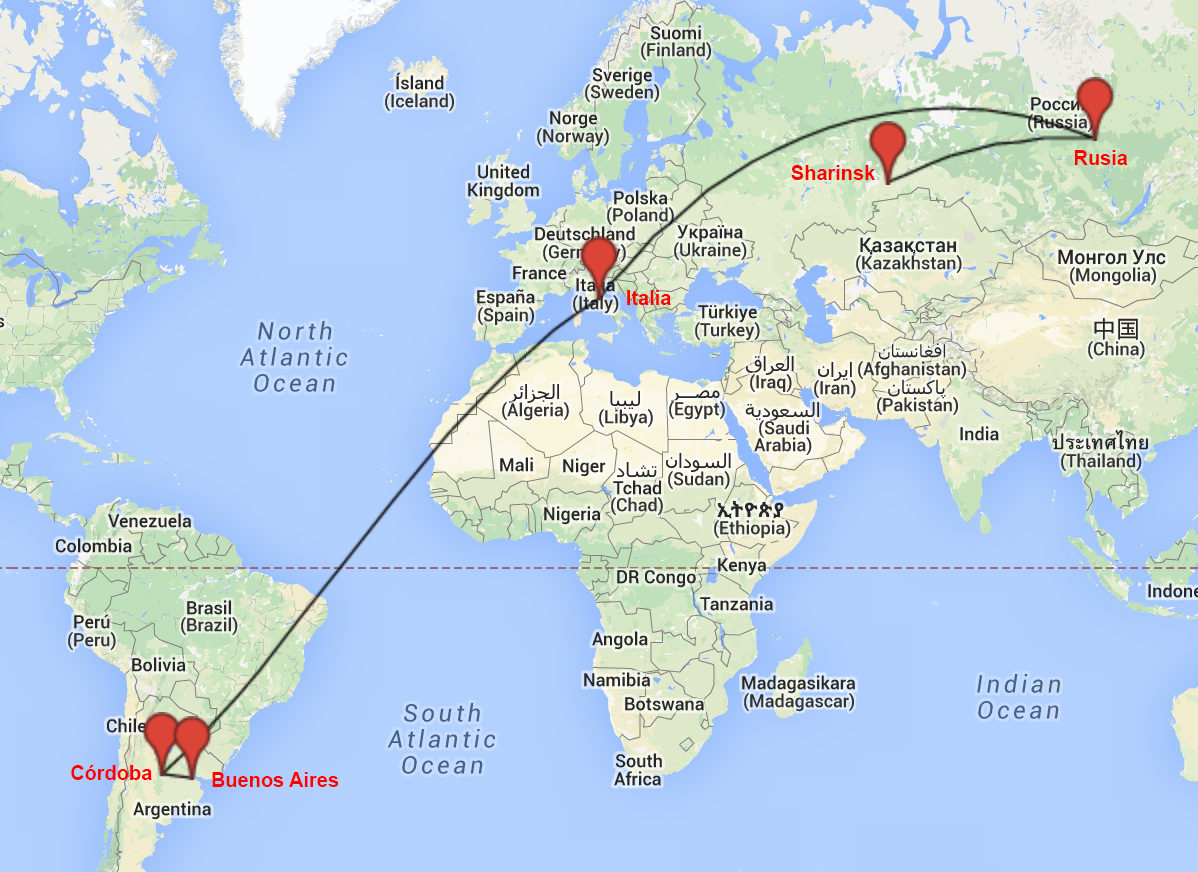
\includegraphics[scale=0.4]{../mapas/mapa_kamgu.png}
		  \caption{Mapa de la ruta atravesada para llegar a la universidad de Kamchatka}
		  \label{fig:contra1}
	\end{center}
\end{figure}

\subsection{Universidad de Japón}

% Please add the following required packages to your document preamble:
% \usepackage{graphicx}
\begin{table}[H]
\resizebox{\textwidth}{!}{%
\begin{tabular}{lllllll}
TTL & IP              & RTT(prom)        & RTT Relativo      & ZRTT                 & Fecha            & Lugar               \\
1   & 192.168.1.1     & 4.37887977151 ms & 4.37887977151 ms  & -0.37903289761414954 & 2014-07-14 22:54 & *                   \\
2   & 190.245.25.1    & 115.919947624 ms & 111.541067853 ms  & 1.6293350395584745   & 2014-07-14 22:54 & Argentina           \\
6   & 200.89.164.141  & 128.567194939 ms & 12.6472473145 ms  & -0.22407222945877223 & 2014-07-14 22:54 & Argentina           \\
7   & 200.89.165.150  & 161.224138737 ms & 32.6569437981 ms  & 0.15093721715367023  & 2014-07-14 22:54 & Argentina           \\
8   & 195.22.220.130  & 166.559362411 ms & 5.33522367477 ms  & -0.361109687323246   & 2014-07-14 22:54 & Italy               \\
9   & 89.221.40.131   & 320.966267586 ms & 154.406905174 ms  & 2.4327002452977204   & 2014-07-14 22:54 & Italy               \\
10  & 89.221.35.186   & 342.196452618 ms & 21.2301850319 ms  & -0.06321608022386131 & 2014-07-14 22:54 & Italy               \\
11  & 61.14.157.93    & 439.377403259 ms & 97.1809506416 ms  & 1.360206539126165    & 2014-07-14 22:54 & Japan               \\
12  & 61.14.158.51    & 464.534175396 ms & 25.1567721367 ms  & 0.010373604579877259 & 2014-07-14 22:54 & Japan               \\
13  & 61.14.158.61    & 450.034415722 ms & -14.4997596741 ms & -0.7328447676290969  & 2014-07-14 22:54 & Japan               \\
14  & 203.192.150.2   & 459.593868256 ms & 9.55945253372 ms  & -0.2819417834993423  & 2014-07-14 22:54 & Asia/Pacific Region \\
15  & 180.145.255.130 & 467.424154282 ms & 7.830286026 ms    & -0.31434876057129946 & 2014-07-14 22:54 & Japan:Osaka         \\
16  & 180.145.253.94  & 488.308882713 ms & 20.8847284317 ms  & -0.06969041573293794 & 2014-07-14 22:54 & Japan:Osaka         \\
17  & 218.228.247.78  & 453.545117378 ms & -34.7637653351 ms & -1.11262032071214    & 2014-07-14 22:54 & Japan               \\
18  & 124.248.144.41  & 450.984311104 ms & -2.56080627441 ms & -0.5090922328908001  & 2014-07-14 22:54 & Japan               \\
19  & 124.248.144.205 & 552.246752907 ms & 101.262441803 ms  & 1.4366993406558966   & 2014-07-14 22:54 & Japan               \\
20  & 210.134.52.222  & 485.796236992 ms & -66.4505159154 ms & -1.7064739461184018  & 2014-07-14 22:54 & Japan               \\
21  & 153.127.246.13  & 458.483612537 ms & -27.3126244545 ms & -0.9729756129298242  & 2014-07-14 22:54 & Japan:Tokyo         \\
22  & 153.127.247.190 & 467.461919785 ms & 8.97830724716 ms  & -0.2928332516679332  & 2014-07-14 22:54 & Japan:Tokyo        
\end{tabular}
}
\caption{Ruta hacia la universidad de Japón. Fecha: 2014-07-14 22:54}
\label{my-label}
\end{table}

% Please add the following required packages to your document preamble:
% \usepackage{graphicx}
\begin{table}[h]
\resizebox{\textwidth}{!}{%
\begin{tabular}{lllllll}
TTL & IP              & RTT(prom)        & RTT Relativo      & ZRTT             & Fecha            & Lugar               \\
1   & 192.168.1.1     & 3.74987721443 ms & 3.74987721443 ms  & -0.294192450162  & 2014-07-15 11:42 & *                   \\
2   & 190.245.25.1    & 19.4438695908 ms & 15.6939923763 ms  & -0.0336452836499 & 2014-07-15 11:42 & Argentina           \\
6   & 200.89.164.141  & 17.0051217079 ms & -2.43874788284 ms & -0.429190205278  & 2014-07-15 11:42 & Argentina           \\
7   & 200.89.165.150  & 17.9165244102 ms & 0.911402702332 ms & -0.356110514524  & 2014-07-15 11:42 & Argentina           \\
8   & 195.22.220.130  & 21.8137145042 ms & 3.89719009399 ms  & -0.290978988734  & 2014-07-15 11:42 & Italy               \\
9   & 89.221.40.131   & 207.880294323 ms & 186.066579819 ms  & 3.68283721068    & 2014-07-15 11:42 & Italy               \\
10  & 89.221.35.186   & 214.749729633 ms & 6.86943531036 ms  & -0.226142869959  & 2014-07-15 11:42 & Italy               \\
11  & 61.14.157.93    & 315.633738041 ms & 100.884008408 ms  & 1.82467716144    & 2014-07-15 11:42 & Japan               \\
12  & 61.14.158.51    & 326.649522781 ms & 11.0157847404 ms  & -0.135695015033  & 2014-07-15 11:42 & Japan               \\
13  & 61.14.158.61    & 324.01124239 ms  & -2.63828039169 ms & -0.433542777997  & 2014-07-15 11:42 & Japan               \\
14  & 203.192.150.2   & 325.588095188 ms & 1.57685279846 ms  & -0.341594484274  & 2014-07-15 11:42 & Asia/Pacific Region \\
15  & 180.145.255.130 & 322.848808765 ms & -2.73928642273 ms & -0.435746108661  & 2014-07-15 11:42 & Japan:Osaka         \\
16  & 180.145.253.94  & 326.363015175 ms & 3.51420640945 ms  & -0.299333338343  & 2014-07-15 11:42 & Japan:Osaka         \\
17  & 218.228.247.78  & 321.682345867 ms & -4.68066930771 ms & -0.478095148581  & 2014-07-15 11:42 & Japan               \\
18  & 124.248.144.41  & 330.128586292 ms & 8.44624042511 ms  & -0.191746675748  & 2014-07-15 11:42 & Japan               \\
19  & 124.248.144.205 & 322.906601429 ms & -7.22198486328 ms & -0.533531031293  & 2014-07-15 11:42 & Japan               \\
20  & 210.134.52.222  & 334.022879601 ms & 11.1162781715 ms  & -0.133502866149  & 2014-07-15 11:42 & Japan               \\
21  & 153.127.246.13  & 329.180902905 ms & -4.84197669559 ms & -0.481613884149  & 2014-07-15 11:42 & Japan:Tokyo         \\
22  & 153.127.247.190 & 327.491104603 ms & -1.68979830212 ms & -0.412852729586  & 2014-07-15 11:42 & Japan:Tokyo        
\end{tabular}
}
\caption{Ruta hacia la universidad de Japón. Fecha: 2014-07-15 11:42}
\label{my-label}
\end{table}

\begin{figure}[H]
	\begin{center}
		  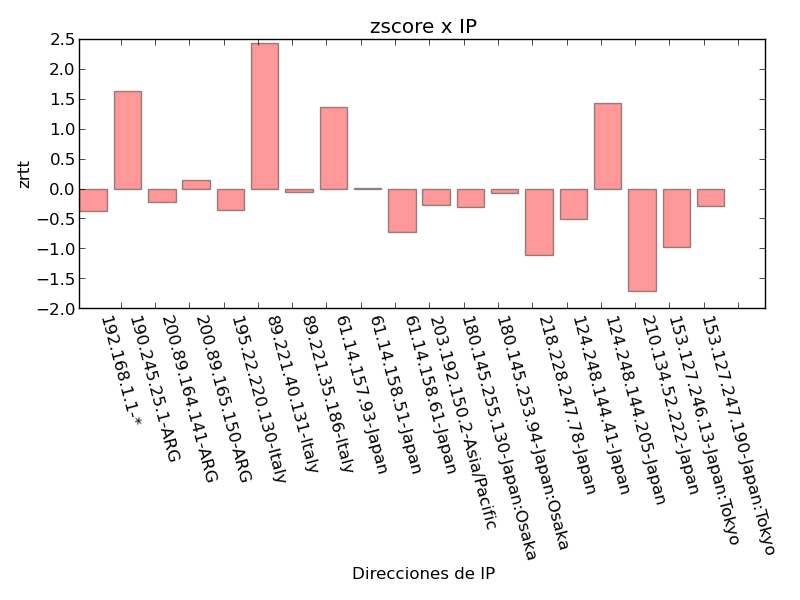
\includegraphics[scale=0.5]{../graficos_informe/jsc_zscore.png}
		  \caption{ZRTT para cada Gateway. Fecha: 2014-07-14 22:54}
		  \label{fig:contra1}
	\end{center}
\end{figure}

\begin{figure}[H]
	\begin{center}
		  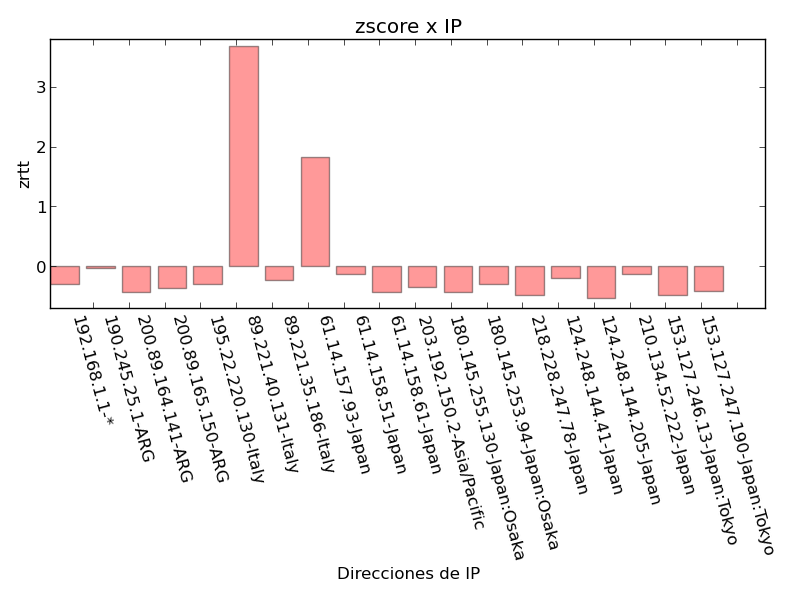
\includegraphics[scale=0.5]{../graficos_informe/jsc_zscore_segunda_medicion.png}
		  \caption{ZRTT para cada Gateway}
		  \label{fig:contra1}
	\end{center}
\end{figure}

%Al igual que para las universidades anteriores puede observarse la gran diferencia del ZRTT antes y luego de pasar el enlace submarino.

%\begin{figure}[H]
%	\begin{center}
%		  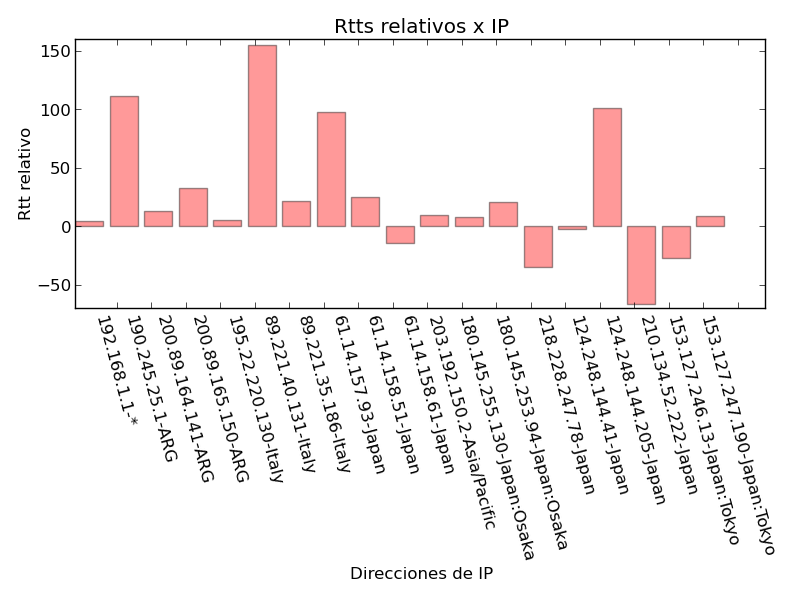
\includegraphics[scale=0.5]{../graficos_informe/jsc_rtt.png}
%		  \caption{RTT relativo para cada Gateway}
%		  \label{fig:contra1}
%	\end{center}
%\end{figure}

\begin{figure}[H]
	\begin{center}
		  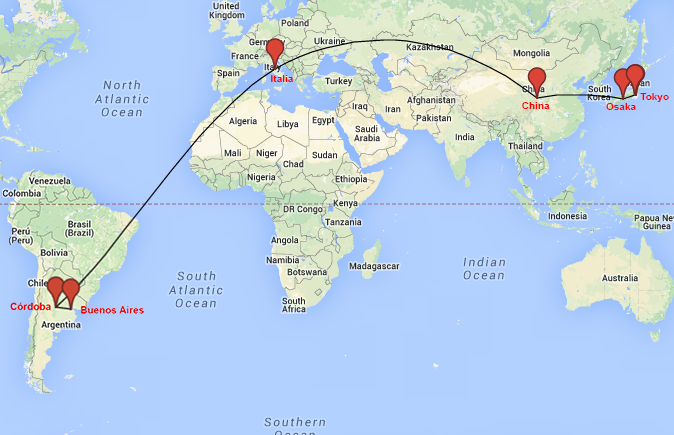
\includegraphics[scale=0.4]{../mapas/mapa_japon.png}
		  \caption{Mapa de la ruta atravesada para llegar a la universidad de Japón}
		  \label{fig:contra1}
	\end{center}
\end{figure}

\subsection{Determinación del umbral}

%Teniendo en cuenta los resultados obtenidos para cada facultad pudimos observar que el valor de ZRTT calculado para cada Gateway definía bastante bien si se trataba de un enlace submarino o no. En la totalidad de los casos evaluados, un valor de ZRTT positivo nos indicaba la presencia de un enlace submarino por lo cual con determinar $u>0$ nos alcanza para detectarlos.


\subsection{Ping vs RTT's calculados}

Para cada facultad decidimos comparar el valor de RTT obtenido por la $tool$ implementada con lo que retorna el comando $ping$. A continuación los resultados:

Ping a Universidad de Australia (2014-07-15 11:29):
\begin{verbatim}
PING www.mq.edu.au (137.111.223.158) 56(84) bytes of data.
64 bytes from survivor.mq.edu.au (137.111.223.158): icmp_req=1 ttl=238 time=391 ms
64 bytes from survivor.mq.edu.au (137.111.223.158): icmp_req=2 ttl=238 time=346 ms
64 bytes from survivor.mq.edu.au (137.111.223.158): icmp_req=3 ttl=238 time=441 ms
64 bytes from survivor.mq.edu.au (137.111.223.158): icmp_req=4 ttl=238 time=371 ms
64 bytes from survivor.mq.edu.au (137.111.223.158): icmp_req=5 ttl=238 time=393 ms
64 bytes from survivor.mq.edu.au (137.111.223.158): icmp_req=6 ttl=238 time=342 ms
64 bytes from survivor.mq.edu.au (137.111.223.158): icmp_req=7 ttl=238 time=378 ms
64 bytes from survivor.mq.edu.au (137.111.223.158): icmp_req=8 ttl=238 time=384 ms
64 bytes from survivor.mq.edu.au (137.111.223.158): icmp_req=9 ttl=238 time=405 ms

\end{verbatim}

Ping a Universidad de Kamchatka (2014-07-15 11:35):

\begin{verbatim}
PING ns.kamgu.ru (85.28.217.202) 56(84) bytes of data.
64 bytes from ns.kamgu.ru (85.28.217.202): icmp_req=1 ttl=48 time=944 ms
64 bytes from ns.kamgpu.ru (85.28.217.202): icmp_req=2 ttl=48 time=958 ms
64 bytes from ns.kamgpu.ru (85.28.217.202): icmp_req=3 ttl=48 time=948 ms
64 bytes from ns.kamgpu.ru (85.28.217.202): icmp_req=4 ttl=48 time=948 ms
64 bytes from ns.kamgpu.ru (85.28.217.202): icmp_req=5 ttl=48 time=949 ms
64 bytes from ns.kamgu.ru (85.28.217.202): icmp_req=6 ttl=48 time=949 ms
64 bytes from ns.kamgpu.ru (85.28.217.202): icmp_req=7 ttl=48 time=948 ms
64 bytes from ns.kamgu.ru (85.28.217.202): icmp_req=8 ttl=48 time=949 ms
64 bytes from ns.kamgu.ru (85.28.217.202): icmp_req=9 ttl=48 time=964 ms
64 bytes from ns.kamgpu.ru (85.28.217.202): icmp_req=10 ttl=48 time=941 ms
64 bytes from ns.kamgu.ru (85.28.217.202): icmp_req=11 ttl=48 time=946 ms
64 bytes from ns.kamgu.ru (85.28.217.202): icmp_req=12 ttl=48 time=970 ms
\end{verbatim}

Ping a Universidad de Japón (2014-07-15 11:42):

\begin{verbatim}
PING jsc.soka.ac.jp (153.127.247.190) 56(84) bytes of data.
64 bytes from v4099.vir.kagoya.net (153.127.247.190): icmp_req=1 ttl=43 time=326 ms
64 bytes from v4099.vir.kagoya.net (153.127.247.190): icmp_req=2 ttl=43 time=345 ms
64 bytes from v4099.vir.kagoya.net (153.127.247.190): icmp_req=3 ttl=43 time=321 ms
64 bytes from v4099.vir.kagoya.net (153.127.247.190): icmp_req=4 ttl=43 time=324 ms
64 bytes from v4099.vir.kagoya.net (153.127.247.190): icmp_req=5 ttl=43 time=368 ms
64 bytes from v4099.vir.kagoya.net (153.127.247.190): icmp_req=6 ttl=43 time=321 ms
64 bytes from v4099.vir.kagoya.net (153.127.247.190): icmp_req=7 ttl=43 time=336 ms
64 bytes from v4099.vir.kagoya.net (153.127.247.190): icmp_req=8 ttl=43 time=323 ms
64 bytes from v4099.vir.kagoya.net (153.127.247.190): icmp_req=9 ttl=43 time=326 ms
\end{verbatim}

Los resultados obtenidos por la $tool$ fueron:

\begin{itemize}
	\item Universidad de Autralia: 343.915832043 ms por la mañana y 447.635984421 ms por la noche.
	\item Universidad de Kamchatka: 947.841417789 ms por la mañana y 959.138429165 ms por la noche.
	\item Universidad de Japón: 327.491104603 ms por la mañana y 467.461919785 ms por la noche.
\end{itemize}

Como es posible observar, los resultados obtenidos por la $tool$ son bastante parecidos a los de $ping$.

\subsection{RTT teórico vs RTT experimental}

Recorrido hasta la universidad de Japón

\begin{itemize}
	\item Buenos Aires - Cordoba: 500km
	\item Cordoba - Italia: 11500km
	\item Italia - China: 7.565km
	\item China - Osaka: 2.832km
	\item Osaka - Tokio: 396km
\end{itemize}

Distancia total: 500+11500+7565+2832+396 = 22793 km
Tiempo de propagación óptimo (Asumiendo links directos entre cada uno de los nodos):
$\frac{22793km}{200000km-s}$ = 0.11 = 110 ms


Recorrido hasta la universidad de Kamgu (Kamchatka)

\begin{itemize}
	\item Buenos Aires - Cordoba: 500km
	\item Cordoba - Italia: 11500km
	\item Italia - Rusia: 5800km
	\item Rusia - Sharinsk:  2100km
\end{itemize}

Distancia total: 500+11500+5800+2100 = 19900
Tiempo de propagación óptimo (Asumiendo links directos entre cada uno de los nodos):
$\frac{19900}{200000km-s}$ = 0.0995 = 99.5 ms


\begin{itemize}
	\item Buenos Aires - Cordoba: 500km
	\item Cordoba - Wichita: 8700km
	\item Wichita - Denver: 700km
	\item Denver - South Australia: 14600km
	\item South Australia - Sidney:  1900km
\end{itemize}

Distancia tota: 500+8700+700+14600+1900 = 26400
Tiempo de propagación óptimo (Asumiendo links directos entre cada uno de los nodos):
$\frac{26400}{200000km-s}$ = 0.132 = 132 ms

Como podemos notar, si todos los enlaces entre los nodos geográficos fueran directos,
asumiendo una velocidad de propagación de los datos equivalente a la de la velocidad
de propagación utilizando fibra óptica \footnote{http://en.wikipedia.org/wiki/Optical\_fiber}, el tiempo que tardarían los paquetes ICMP en llegar a destino sería similar en los 3 casos. (Entre 100 y 132 ms). Como era de esperarse, este tiempo teórico óptimo es bastante menor al obtenido experimentalmente. Sin embargo se encuentra en el mismo orden de magnitud.


















